\documentclass[open=left,twopage=true]{scrreprt}

\usepackage{xspace}
\usepackage{amsmath}
\usepackage{amssymb}
\usepackage{latexsym}
\usepackage{pgf}
\usepackage{pgfarrows}
\usepackage{ntheorem}
\usepackage{lscape}
\usepackage{graphicx}
\usepackage{epic,eepic}
\usepackage{tikz}
\usetikzlibrary{automata,calc,shapes.geometric,arrows,shadings,chains}

\input{./makros}
\definecolor{darkgreen}{rgb}{.1,.6,.1}
\definecolor{darkred}{rgb}{.6,.1,.1}

\definecolor{light-blue}{rgb}{0.7,0.8,1}
\usepackage[allbordercolors={light-blue},pdfborderstyle={/S/U/W 0.8}]{hyperref}

\begin{document}

\begin{titlepage}
%\subject{Report}
\title{The \pgsolver Collection of Parity Game Solvers \\[2mm] {\large Version 4.2}}
\author{Oliver Friedmann \\ \normalsize Institut f\"ur Informatik \\ \normalsize Ludwig-Maximilians-Universit\"at M\"unchen, Germany \and 
Martin Lange \\ \normalsize Theoretical Computer Science / Formal Methods \\ \normalsize School of Electr.\ Eng.\ and Computer Science \\ 
\normalsize University of Kassel, Germany}
\publishers{
\vspace*{1cm}
\scalebox{0.8}{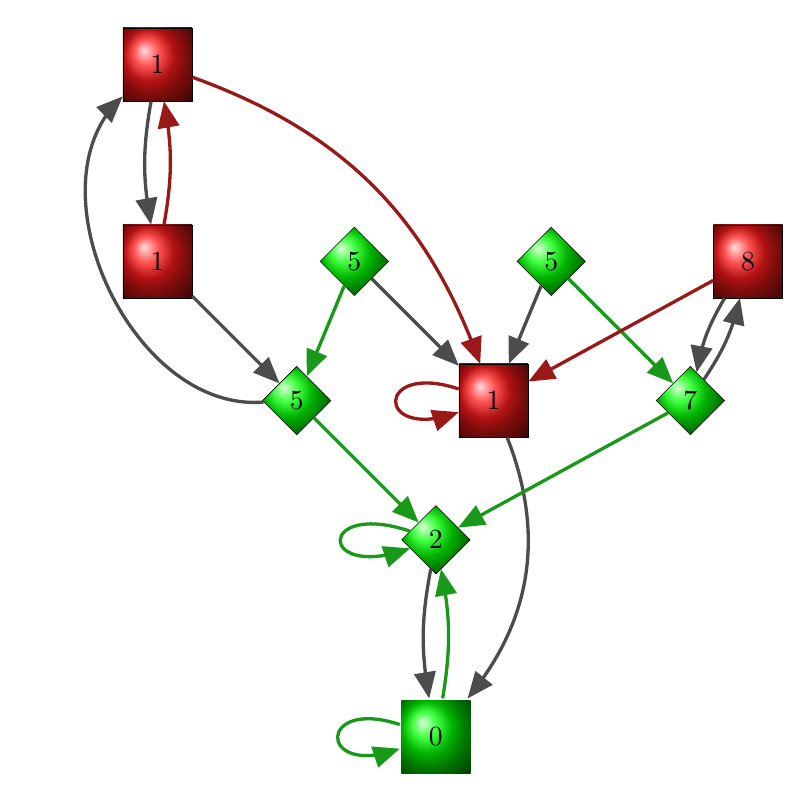
\begin{tikzpicture}[very thick,node distance=2.5cm,-triangle 45]
%\scalebox{0.59}{\includegraphics{graphics/titlegame}}

  \tikzstyle{redboxnode}=[draw=black,very thin,shape=rectangle,inner sep=10pt,ball color=red!90,shading=ball]
  \tikzstyle{reddiamnode}=[draw=red,shape=diamond]
  \tikzstyle{greenboxnode}=[shape=rectangle,inner sep=10pt,ball color=green,shading=ball]
  \tikzstyle{greendiamnode}=[draw=black,very thin,shape=diamond,ball color=green,shading=ball]

  \node[redboxnode]    (v0)                     {$1$};
  \node[redboxnode]    (v1) [below of=v0]       {$1$};
  \node[greendiamnode] (v2) [right of=v1]       {$5$};
  \node[greendiamnode] (v3) [right of=v2]       {$5$};
  \node[redboxnode]    (v4) [right of=v3]       {$8$};
  \node[greendiamnode] (v5) [below right of=v1] {$5$};
  \node[redboxnode]    (v6) [below right of=v2] {$1$};
  \node[greendiamnode] (v7) [below right of=v3] {$7$};
  \node[greendiamnode] (v8) [below right of=v5] {$2$};
  \node[greenboxnode]  (v9) [below of=v8]       {$0$};

  \path[black!70] (v0) edge [bend right=10] (v1)
                  (v1) edge                 (v5)
                  (v2) edge                 (v6)
                  (v3) edge                 (v6)
                  (v4) edge [bend right=10] (v7)
                  (v5) edge [bend left=70]     (v0)
                  (v6) edge [bend left]     (v9) 
                  (v7) edge [bend right=10] (v4)
                  (v8) edge [bend right=10] (v9);

  \draw[darkgreen] (v2) edge                 (v5)
                   (v3) edge                 (v7)
                   (v5) edge                 (v8)
                   (v7) edge                 (v8)
                   (v9) edge [bend right=10] (v8);

  \draw[darkred] (v0) edge [bend left=25]  (v6)
                 (v1) edge [bend right=10] (v0)
                 (v4) edge                 (v6);

  \draw[darkgreen] (v8) .. controls ($(v8)+(-1.5,.5)$) and ($(v8)+(-1.5,-.5)$) .. (v8);
  \draw[darkgreen] (v9) .. controls ($(v9)+(-1.5,.5)$) and ($(v9)+(-1.5,-.5)$) .. (v9);
  \draw[darkred]   (v6) .. controls ($(v6)+(-1.5,.5)$) and ($(v6)+(-1.5,-.5)$) .. (v6);

\end{tikzpicture}}}
\end{titlepage}
\maketitle[0]

\cleardoublepage
\pdfbookmark{Contents}{table-of-contents}
\tableofcontents

\chapter{Introduction}

\input{./intro}

\chapter{Solving Parity Games}
\label{chp:pgames}

\input{./tech}
\input{./locglob}
\input{./verify}
\input{./univopt}
\input{./gensolv}
\input{./implalg}
\input{./implheur}

\chapter{User's Guide}
\label{chp:uguide}

\section{License}

This software is distributed under the BSD license.
\begin{verbatim}
Copyright (c) 2008-2021 Oliver Friedmann and Martin Lange
All rights reserved.

Redistribution and use in source and binary forms, with or without
modification, are permitted provided that the following conditions
are met:
1. Redistributions of source code must retain the above copyright
   notice, this list of conditions and the following disclaimer.
2. Redistributions in binary form must reproduce the above copyright
   notice, this list of conditions and the following disclaimer in the
   documentation and/or other materials provided with the distribution.
3. The name of the author may not be used to endorse or promote products
   derived from this software without specific prior written permission.

THIS SOFTWARE IS PROVIDED BY THE AUTHOR ``AS IS'' AND ANY EXPRESS OR
IMPLIED WARRANTIES, INCLUDING, BUT NOT LIMITED TO, THE IMPLIED WARRANTIES
OF MERCHANTABILITY AND FITNESS FOR A PARTICULAR PURPOSE ARE DISCLAIMED.
IN NO EVENT SHALL THE AUTHOR BE LIABLE FOR ANY DIRECT, INDIRECT,
INCIDENTAL, SPECIAL, EXEMPLARY, OR CONSEQUENTIAL DAMAGES (INCLUDING, BUT
NOT LIMITED TO, PROCUREMENT OF SUBSTITUTE GOODS OR SERVICES; LOSS OF USE,
DATA, OR PROFITS; OR BUSINESS INTERRUPTION) HOWEVER CAUSED AND ON ANY
THEORY OF LIABILITY, WHETHER IN CONTRACT, STRICT LIABILITY, OR TORT
(INCLUDING NEGLIGENCE OR OTHERWISE) ARISING IN ANY WAY OUT OF THE USE OF
THIS SOFTWARE, EVEN IF ADVISED OF THE POSSIBILITY OF SUCH DAMAGE.
\end{verbatim}

%%% Local Variables:
%%% mode: latex
%%% TeX-master: "main"
%%% End:

\section{Change Log}

Changes are classified according to their importance. Changes effecting only the performance of
parts of the tool or are less important otherwise are marked with one asterisk ($\ast$). Changes
that are worth noting like the addition of new features etc.\ are marked with two asterisks 
($\ast\ast$). Finally, major changes that would effect usability, for example breaks in backwards
compatibility, changes in the user interface, etc., are marked with three asterisks ($\ast\ast\ast$).

Changes incorporated into version 4.2:
\begin{itemize}
\item[$\ast$] Removed dependency on deprecated OCaml Pervasives module.
\end{itemize}

Changes incorporated into version 4.1:
\begin{itemize}
\item[$\ast\ast$] \pgsolver is now built using \texttt{opam} and \texttt{oasis}. No more git submodules are in use.
\end{itemize}

Changes incorporated into version 4.0:
\begin{itemize}
\item[$\ast\ast\ast$] The interface and implementation of the module \texttt{Paritygame} have undergone some major changes,
     mostly concerning the data types for parity games. This type is now abstract, so access to and manipulations of parity games
     are now only possible through specialised functions in this module. A direct access of parity games as arrays is no longer
     possible. Consequently, access to parity games in all other modules has been changed accordingly. This encapsulation step 
     enables us to change the internal data structures for parity games easily for optimisation purposes without changing any of 
     the algorithms around them. It is also worth noticing that a node in a parity game now knows its predecessors as well as its
     successors. Hence, functions for computing transposed graphs etc.\ have been removed.
\item[$\ast\ast$] \pgsolver is now built using \texttt{ocamlbuild}. It requires the OCaml packages \texttt{ocamlfind} and \texttt{ounit}.
     Get them using \texttt{opam}. Moreover, \pgsolver now requires OCaml version 4.03.0.
\item[$\ast\ast\ast$] If a textual presentation of a parity game starts with the keyword \texttt{parity} then it is followed by the number of
     nodes in the game, rather than the largest identifier of a node in the game. So any ``\texttt{parity} $n$'' should now be 
     ``\texttt{parity} $n+1$''.
\item[$\ast$] A framework for the easy creation of benchmarks derived from model-checking problems is now provided. 
\item[$\ast\ast$] Support for the \texttt{Z3} has been discontinued.  
\end{itemize}

Changes incorporated into version 3:
\begin{itemize}
\item[$\ast\ast$] \pgsolver is now linkable as library.
\item[$\ast$] A new local strategy improvement algorithm has been added.
\item[$\ast\ast$] Local Solving of Games has been enabled.
\item[$\ast$] Generators can now be linked directly into \pgsolver.
\item[$\ast$] Two new randomized strategy improvement algorithms have been incorporated.
\item[$\ast$] The lists of solvers and generators are now maintained in \texttt{./Solvers} and \texttt{./Generators} respectively.
\item[$\ast$] Printing and parsing of solution and strategies.
\item[$\ast$] Conversion between min-parity and max-parity games as a new transformer feature.
\item[$\ast$] Two new generators: Towers of Hanoi as a reachability game and a fairness verification of an elevator system.
\end{itemize} 



Changes incorporated into version 2:
\begin{itemize}
\item[$\ast$] In order to allow more efficient parsing, the specification format for parity
      games has been extended. It is now possible to include at the beginning of the specification
      the maximal index of a node in the game. If this is done, then parsing will be quicker.
\item[$\ast$] All the random game generators are now based on a more efficient generation
      of sets of random numbers.
\item[$\ast$] The computation of attractor regions has been improved.
\item[$\ast\ast\ast$] Confusing terminology has been clarified: the algorithm due to Stevens and
     Stirling \cite{StevensStirling98} is now referred to as the \emph{model checker} rather than the 
     former \emph{game-based algorithm}. Command line parameters to \texttt{pgsolver} have been 
     changed accordingly.
\item[$\ast\ast$] A useful benchmarking tool has been included in the distribution.
\item[$\ast$] This change log has been included in this documentation -- in case you hadn't noticed.
\end{itemize} 

 

%%% Local Variables: 
%%% mode: latex
%%% TeX-master: "main"
%%% End: 

\section{Installation Guide}

\subsection{Obtaining the Relevant Parts}

You can obtain the source code for \pgsolver from
\begin{center}
    \url{https://github.com/tcsprojects/pgsolver}
\end{center}
Download the latest sources.
\begin{verbatim}
    ~> git clone https://github.com/tcsprojects/pgsolver
\end{verbatim}
This will create a directory \texttt{pgsolver} and various subdirectories in it.
\begin{verbatim}
    ~> cd pgsolver
\end{verbatim}

In order to compile \pgsolver from source code you will need the OCaml compiler. A convenient way is to install the OCaml 
Package Manager \texttt{opam}. Install it via any package manager for your system or download it from
\begin{center}
\url{https://opam.ocaml.org/}
\end{center}
Then get the OCaml compiler installed via.
\begin{verbatim}
    ~> opam switch 4.07.0 
    ~> eval `opam config env`
\end{verbatim}
It may be recommendable to use a later version of the OCaml compiler. Previous versions before 4.07.0 may also work.

Next you need the compilation tool \texttt{ocamlbuild} and some additional packages which can be installed via:
\begin{verbatim}
    ~> opam install ocamlbuild ocamlfind TCSLib extlib ocaml-sat-solvers minisat
\end{verbatim}

If you intent to contribute to the development of \pgsolver you may want to use unit tests as well. This requires:
\begin{verbatim}
    ~> opam install ounit
\end{verbatim}



\subsection{Compiling \pgsolver}

Now change into the \pgsolver directory.
\begin{verbatim}
    ~> cd pgsolver
\end{verbatim}

To start the compilation, type 
\begin{verbatim}
    ~/pgsolver> ocaml setup.ml -configure
    ~/pgsolver> ocaml setup.ml -build
\end{verbatim}


\section{Running \pgsolver}

\subsection{Invocation}

A successful compilation produces an executable binary called \texttt{pgsolver} which
resides in the subdirectory \texttt{bin}. Type
\begin{verbatim}
    ~/pgsolver> bin/pgsolver --help
\end{verbatim}
or
\begin{verbatim}
    ~/pgsolver> bin/pgsolver -help
\end{verbatim}
for a list of command-line options and a description of the command-line parameters that the
program expects.

The specification of the parity game to be solved -- cf.\ Sect.~\ref{sec:specs} -- can either be
given in a file or through \texttt{stdin}. The latter case is the default, and to switch to the
former one only needs to give the name of the file including the specification as a command-line
argument.
\begin{verbatim}
    ~/pgsolver> bin/pgsolver tests/test1.gm
\end{verbatim}

\subsection{Command-Line Parameters}

\pgsolver's behaviour can be changed through command-line parameters. In particular, you can determine
the algorithm that is used for solving, specify whether or not you want to view the result in text
mode or graphically, etc. Command-line parameters can be given in any order, although some are
conflicting and in that case the latter overrides the former; for example when you specify more than
one algorithm that should be used for solving. The currently understood command-line parameters are:
\begin{description}
\itemsep3mm
\item[\nonterminal{filename}] \ \\
   Tells \texttt{pgsolver} to look for the specification of the parity game to solve in the file
   \nonterminal{filename}.

\item[{\ttfamily  -v \nonterminal{level}}] \ \\
   Sets the verbosity level, valid arguments are $0$--$3$, the default is 1. With verbosity level $0$,
   \texttt{pgsolver} will be very humble and not bother \texttt{stdout} with its pathetic goobledigook.
   With verbosity level 1, it will tell you what it does and what the winning regions and strategies
   are. With verbosity level 2, it will tell you a bit more, but this very much depends on which
   algorithm is chosen for solving etc. It may for example tell you something it has found out about the
   SCC structure or priority distribution in the game. Verbosity level 3 is for debugging purposes. Again,
   this very much depends on the solving algorithm.

%\item[{\ttfamily --quiet}] \ \\
%   Causes the program to be quiet, same as \texttt{-v 0}.

%\item[{\ttfamily --verbose}] \ \\
   %Causes the program to be verbose, same as \texttt{-v 2}.

%\item[{\ttfamily --debug}] \ \\
   %Causes the program to be very verbose, same as \texttt{-v 3}.

\item[{\ttfamily -d \nonterminal{filename}}] \ \\
   Tells \texttt{pgsolver} to open the file \nonterminal{filename} for writing and print into it the
   \texttt{dot}-code of the parity game as a graph, see also Sect.~\ref{sec:viewing}. If the game has
   been solved during this invocation then the graphical presentation will display the winning regions
   and strategies. You can use option \texttt{-n} in combination with this one to display a pure parity
   game, i.e.\ without the winning information.

% \item[{\ttfamily -f}] \ \\
%    Causes \texttt{pgsolver} to print the whole game on \texttt{stdout} again. The format is the one
%    that \texttt{pgsolver} would expect as input.\TODO{Hat das einen besonderen Sinn?}

% \item[{\ttfamily --sanitycheck}]  \enspace or {\ttfamily -sc} \\
%   Checks whether the given parity game is well-formed, meaning that it particularly does not contain any edge leading to inaccessible nodes.

% \item[{\ttfamily -n}] \ \\
%    Tells \texttt{pgsolver} to suppress solving. This can be used to simply draw a parity game in
%    \texttt{dot}-format without the information about winning regions and strategies. This is a default
%    selection, i.e.\ \pgsolver will not solve a game unless you specify explicitly which algorithm it
%    should use. See below for the command-line parameters that let you do so.

\item[{\ttfamily --disableglobalopt}]  \enspace or {\ttfamily -dgo} \\
   Tells \texttt{pgsolver} to completely disable any global optimisations. Global optimisation is enabled by default.

% \item[{\ttfamily --disableuselesscycles}]  \enspace or {\ttfamily -dul} \\
%    Tells \texttt{pgsolver} to disable to automatic deletion of useless self cycles. This is a global optimisation and is enabled by default.
% 
% \item[{\ttfamily --disableusefulcycles}]  \enspace or {\ttfamily -duf} \\
%    Tells \texttt{pgsolver} to disablee the automatic utilisation of useful self cycles. This is a global optimisation and is enabled by default.

\item[{\ttfamily --disablesccdecomposition}]  \enspace or {\ttfamily -dsd} \\
   Tells \texttt{pgsolver} to decompose the game into strongly connected components. This is enabled by default.

\item[{\ttfamily --disablelocalopt}]  \enspace or {\ttfamily -dlo} \\
   Tells \texttt{pgsolver} to completely disable any local optimisations. Local optimisation is enabled by default.

% \item[{\ttfamily --enableprioprop}]  \enspace or {\ttfamily -pp} \\
%    Tells \texttt{pgsolver} to enable priority propagation. This is a local optimisation and is disabled (!) by default.
% 
% \item[{\ttfamily --disablepriocomp}]  \enspace or {\ttfamily -dcp} \\
%    Tells \texttt{pgsolver} to disable priority compression. This is a local optimisation and is enabled by default.

\item[{\ttfamily --disablespecialgames}]  \enspace or {\ttfamily -dsg} \\
   Tells \texttt{pgsolver} to completely disable any algorithms solving special instances. This is enabled by default.

% \item[{\ttfamily --disablesingleparity}]  \enspace or {\ttfamily -dpa} \\
%    Tells \texttt{pgsolver} to disable the automatic solving of single parity instances. This is a special instance solving optimisation and is enabled by default.
% 
% \item[{\ttfamily --disablesingleplayer}]  \enspace or {\ttfamily -dpl} \\
%    Tells \texttt{pgsolver} to disable the automatic solving of single player instances. This is a special instance solving optimisation and is enabled by default.

\item[{\ttfamily --verify}]  \enspace or {\ttfamily -ve} \\
   This causes \texttt{pgsolver} to perform, after solving, an additional check that the reported winning
   strategies are correct; useful for finding bugs in new algorithm implementations.

% \item[{\ttfamily --verify2}]  \enspace or {\ttfamily -ve} \\
%    Same as {\ttfamily --verify} but use a different verification method; useful for finding bugs in new
%    algorithm implementations if you have used \texttt{--verify} but want to be really sure.
% 
% \item[{\ttfamily --verify3}]  \enspace or {\ttfamily -ve} \\
%    Still the same as {\ttfamily --verify} or {\ttfamily --verify2} but uses yet again a different verification method;
%    useful for finding bugs in new algorithm implementations if you have used \texttt{--verify} and
%    \texttt{--verify2} but generally have issues with trust.

\item[{\ttfamily --justheatCPU}] \enspace or {\ttfamily -jh}  \\
   On large parity games, printing the winning information can take a long time because of the bottleneck
   \texttt{stdout}. This option turns the printing of that information off. Useful if one is interested in
   running times only for instance.

\item[{\ttfamily --changesat \nonterminal{satsolver}}] \enspace or {\ttfamily -cs \nonterminal{satsolver}}  \\
   Selects the SAT solver backend that is to be used. Only affects parity game solving algorithms that
   depend on SAT solving. If there are less than two SAT solvers linked into \pgsolver, this parameter
   is disabled.

\item[{\ttfamily --printsolonly}] \enspace ${}$ \\
	Instead of printing a human readable form of the solution, \pgsolver prints a
	format that can be directly parsed again by the framework.

\item[{\ttfamily --printsolvedgame}] \enspace or {\ttfamily -pg} \\
	Prints the solved game in a parseable form. This will be a subgame of the
	original parity game in which all nodes where the winner of the node is also
	the owner are restricted to the winning edge.

\item[{\ttfamily --parsesolution \nonterminal{file}}] \enspace or
{\ttfamily -ps \nonterminal{file}}  \\
	Parses a previously printed solution into \pgsolver. This allows you to, for
	instance, verify a particular solution.

\item[{\ttfamily --solverinfo}] \enspace  ${}$ \\
	Prints out a list of all available solvers.

\item[{\ttfamily --globallysolve \nonterminal{solver}}] \enspace or
{\ttfamily -global \nonterminal{solver}}  \\
	Chooses a particular global solver to solve the game at hand.

\item[{\ttfamily --locallysolve \nonterminal{solver} \nonterminal{node}}]
\enspace or {\ttfamily -local \nonterminal{solver} \nonterminal{node}}  \\
	Chooses a particular local solver to solve the game at hand starting from a
	specified node.

\item[{\ttfamily --args \nonterminal{arguments}}] \enspace or
{\ttfamily -x \nonterminal{arguments}}  \\
	Provides additional arguments to a solvers. You can get the full list of
	arguments for a particular solver by calling \pgsolver with {\ttfamily -x
	"help"}.

\item[{\ttfamily --generator \nonterminal{generator} \nonterminal{arguments}}]
\enspace or {\ttfamily -gen \nonterminal{generator} \nonterminal{arguments}}  \\
	Generates a game using one of the included generators directly for \pgsolver to
	solve.


% 
% \item[{\ttfamily --viasat}] \enspace or {\ttfamily -vs} \\
%    Use the small progress measure encoding for propositional logic and a reduction to SAT due to Lange.
%    Also see the command-line parameters that select the SAT solver to be used.
%    This parameter is only available if there is at least one SAT solver linked into \pgsolver.
% 
% \item[{\ttfamily --stratimprove}] \enspace or {\ttfamily -si} \\
%    Use the strategy improvement algorithm due to Jurdzi{\'n}ski and V\"oge.
% 
% \item[{\ttfamily  --optstratimprov}] \enspace or {\ttfamily -os} \\
%    Use the strategy improvement algorithm due to Schewe.
% 
% \item[{\ttfamily --smallprog}] \enspace or {\ttfamily -sp} \\
%    Use the small progress measure algorithm due to Jurdzi{\'n}ski.
% 
% \item[{\ttfamily --satsolve}] \enspace or {\ttfamily -ss} \\
%    Tells \texttt{pgsolver} to encode a direct NP predicate that is to be solved due To Friedmann.
%    This parameter is only available if there is at least one SAT solver linked into \pgsolver.
% 
% \item[{\ttfamily --recursive}] \enspace or {\ttfamily -re} \\
%    Use the recursive algorithm due to Zielonka.
% 
% \item[{\ttfamily --modelchecker}] \enspace or {\ttfamily -mc}  \\
%    Use the $\mu$-calculus model checker due to Stevens and Stirling.
% 
% \item[{\ttfamily --dominiondec}] \enspace or {\ttfamily -dd} \\
%    Use the dominion decomposition algorithm due to Jurdzi{\'n}ski, Paterson, and Zwick.
% 
% \item[{\ttfamily --bigstep}] \enspace or {\ttfamily -bs} \\
%    Use the big-step procedure due to Schewe.
% 
% \item[{\ttfamily --guessstrategy}] \enspace or {\ttfamily -gs} \\
%    Use the strategy guessing heuristic.

\end{description}



\subsection{Output}

An invocation of
\begin{verbatim}
    ~/pgsolver> bin/randomgame 10 10 2 4 | bin/pgsolver -global recursive
\end{verbatim}
will typically create output on \texttt{stdout} like this:
\begin{verbatim}
    Parsing ....................... 0.00 sec
    Chosen solver `recursive' ..... 0.00 sec

    Player 0 wins from nodes:
      {0,2,5,6,7,8}
    with strategy
      [0->6,2->2,5->0,6->2,7->7,8->8]

    Player 1 wins from nodes:
      {1,3,4,9}
    with strategy
      [1->9,3->9,4->3,9->9]
\end{verbatim}
It reports the times it took to parse the input and to solve the game specified in this input
as well as which solver has been used. Then it reports for both players the sets of winning
regions in the game as a list of natural numbers (each node's index in the game) in ascending order.
The positional strategies are reported as a list of pairs of the form $x$\texttt{->}$y$ meaning
that in node $x$, the player at hand should move to node $y$. This list is also sorted in
ascending order w.r.t.\ $x$. Furthermore, the set of nodes given as $x$'s in this list is
exactly the set of nodes belonging to that player.




%%% Local Variables:
%%% mode: latex
%%% TeX-master: "main"
%%% End:

\input{./specs}
\input{./display}
\input{./tools}

\chapter{Benchmarks}
\label{chp:benchmarks}

% !TEX root =  main.tex

%\section{Benchmark Games}

%The \pgsolver library contains a few programs that create benchmarks for the parity game
%solvers. They are built using the command
%\begin{verbatim}
%    ~/pgsolver> make generators
%\end{verbatim}
%and reside afterwards in the subdirectory \texttt{bin}.
%
%Additionally, it is possible to compile all generators directly into \pgsolver by setting
%the variable \texttt{LINKGENERATORS} to \texttt{YES} in the \texttt{./Config}-file. This
%has the advantage that the process of generating and solving a game is not slowed down by
%formatting the game first and parsing it afterwards again into the same data structure.

\section{Random Games}

\subsection{A Na\"{\i}ve Model}
Randomly generated parity games are the simplest form of benchmarking utility to assess the
performance of game solvers. The ones used here are parametrized by four parameters: the number
$n$ of nodes in the game, the highest priority $p$, a lower and an upper bound $l$ and $u$ on the
out-degree of each node. The call
\begin{verbatim}
    ~/pgsolver> bin/randomgame 1000 200 2 5
\end{verbatim}
creates a random game with 1000 nodes as follows: for each node $v$,
\begin{itemize}
\item the priority $\Omega(v)$ is uniformly chosen among $\{0,\ldots,200\}$;
\item node $v$ belongs to player $0$ with probability $0.5$ and therefore to player $1$ with
      probability $0.5$ as well;
\item a number $d$ is uniformly chosen in the range $\{2,\ldots,5\}$, and $d$ pairwise different
      nodes are uniformly chosen as $v$'s successors.
\end{itemize}
Beware that \texttt{bin/randomgame} may crash or not terminate if 
\begin{itemize}
\item the lower bound on the outdegree is greater than the upper bound,
\item the lower bound is smaller than $1$, or
\item the upper bound is greater than the number of nodes.
\end{itemize}


\subsection{Clustered Random Games}

Almost every game created by the random generator above consists of a single big SCC and many adhesive
chains.

Therefore this generator uses an other random model that accomplishes to bring a bit more structure into its instances. It depends on nine parameters: The number of nodes $n$, the highest possibly occurring priority $p$, an out-degree range $(l;h)$, a recursion depth $r$, a recursion breadth range $(a;b)$ and an interconnection range $(x;y)$. An instance of $\mathcal{G}^c_{(n,r)}$ with $c = (p,l,h,a,b,x,y)$ can be generated as follows. If $r = 0$ or $a > n$ simply return a randomly generated game with $n$ nodes, highest priority $p$ and out-degree bounds $l$ and $h$ as above. If $r > 0$ and $a \leq n$,
\begin{itemize}
\item a number $d$ is uniformly chosen in the range $\{a,\ldots,\min(b,n)\}$;
\item $d$ numbers $k_0,\ldots,k_{d-1}$ are uniformly chosen in the range $\{0,\ldots,n-1\}$ s.t.\ $\sum_{i=0}^{d-1} k_i = n$;
\item $d$ instances $G_0,\ldots,G_{d-1}$ are chosen, where $G_i$ is chosen from $\mathcal{G}^c_{(k_i,r-1)}$ (we assume the nodes of all $G_i$ to be pairwise different);
\item a game $G$ is created by the union of all $G_i$;
\item a number $e$ is uniformly chosen in the range $\{x,\ldots,y\}$;
\item $e$ additional uniformly chosen edges in $G$ are added to $G$;
\item the game $G$ is returned.
\end{itemize}

Basically, this recursive approach creates a topological tree structure that is partially intercepted by adding the additional interconnection edges.

A clustered random game with 1000 nodes, highest priority 2, out-degree bounds 2 and 5, recursion depth 3, recursion breadth between 4 and 6 and interconnection degree between 11 and 22 is created using the call
\begin{verbatim}
    ~/pgsolver> bin/clusteredrandomgame 1000 200 2 5 3 4 6 11 22
\end{verbatim}


\subsection{Steady Random Games}

The Steady Random Generator tries to circumvent many universal optimisations in order to particularly
benchmark the backend solvers. The Steady Random Generator is parametrized by five parameters: the number
$n$ of nodes (and different priorities) in the game, a lower and an upper bound and on the
out-degree of each node and a lower and an upper bound and on the in-degree of each node. The call
\begin{verbatim}
    ~/pgsolver> bin/steadygame 1000 2 4 3 5
\end{verbatim}
creates a random game with 1000 nodes as follows: for each node $v$,
\begin{itemize}
\item the priority $\Omega(v)$ is simply $v$;
\item node $v$ belongs to player $0$ with probability $0.5$ and therefore to player $1$ with
      probability $0.5$ as well;
\item a number $d$ is uniformly chosen in the range $\{2,\ldots,4\}$, and $d$ pairwise different
      nodes are uniformly chosen in $v$'s subgame as $v$'s successors;
\item a number $d$ is uniformly chosen in the range $\{3,\ldots,5\}$, and an attempt is made to ensure
      that $v$ has $d$ pairwise different predecessors.
\end{itemize}
All edges are iteratively determined as long as there are at least two different nodes with one of them violating
a lower bound and the other one being below the opposite upper bound uniformly between two such nodes.


\section{Special Graph Structures}

\subsection{Clique Games}

The clique game of order $n$ is $G_n = (\{0,\ldots,n-1\},\{0,2,4,\ldots\},\{1,3,5,\ldots\},E,\Omega)$
with $E = \{ (v,w) \mid v \ne w \}$ and $\Omega(v) = v$. It forms a clique in a directed graph without
self-cycles. Clique games exhibit a large amount of cycles in the game which may pose difficulties
for certain solvers. Note that adding self-cycles to the nodes will result in easy solving because
self-cycles are partial winning strategies in this case, and then all other nodes would lie in the attractor
of these winning regions.

The clique game of order $50$ for instance is generated as follows.
\begin{verbatim}
    ~/pgsolver> bin/cliquegame 50
\end{verbatim}
The clique game of order 50 with self-cycles can also be generated.
\begin{verbatim}
    ~/pgsolver> bin/cliquegame 50 self
\end{verbatim}


\subsection{Ladder Games}
\label{sec:laddergame}

The name of these games is derived from their structure which is reminiscent of a ladder. The
\emph{ladder game} of index $n$ is $G_n = (V,V_0,V_1,E,\Omega)$, defined as follows.
\begin{itemize}
\item $V = \{0,\ldots,2n-1\}$,
\item $V_0 = \{0,2,4,\ldots,2n-2\}$, $V_1 = \{1,3,5,\ldots,2n-1\}$,
\item $E = \{ (v,w) \mid w \equiv_{2n} v+i $ for some $i \in \{1,2\}$ $\}$,
\item $\Omega(v) = v \mod 2$.
\end{itemize}
where $\equiv_{2n}$ means equality modulo $2n$.

It is not hard to see that player $0$ wins on $V_0$ and player $1$ wins on $V_1$ since both can
stay within these regions and only see the priorities $0$, resp.\ $1$.

Ladder games are chosen as benchmarks because in $G_n$ there are $2^n$ many positional strategies for each
player but only one of them is a winning strategy. Not surprisingly, ladder games are very difficult
to solve for the strategy guessing heuristic for example.

The ladder game of index 19 is created using the call
\begin{verbatim}
    ~/pgsolver> bin/laddergame 19
\end{verbatim}


\section{Hard Games for Particular  Algorithms}


\subsection{Jurdzi{\'n}ski Games}
\label{sec:jurdgame}

Jurdzi{\'n}ski has defined a family of games on which the small progress measures algorithm
exhibits an exponential running time \cite{Jurdzinski/00}. The Jurdzi{\'n}ski game $J_{d,w}$ of depth 
$d$ and width $w$ forms a rectangle of dimension $(2d+1) \times (2w)$. For instance, $J_{50,100}$
is generated by calling
\begin{verbatim}
    ~/pgsolver> bin/jurdzinskigame 50 100
\end{verbatim}


% \begin{figure}[t]
% \begin{center}
% \scalebox{0.6}{\input{graphics/marcingame.eepic}}
% \end{center}

% \caption{The Jurdzi{\'n}ski games.}
% \label{fig:marcingame}
% \end{figure}



\subsection{Recursive Ladder Games}

%\include{pgfgraphics}

% \begin{figure}[t]
% \begin{center}
% \pictrecursiveladder
% \end{center}
% \caption{The recursive ladder game of index 4.}
% \label{fig:recursiveladder}
% \end{figure}

The recursive ladder games form a family on which the recursive algorithm exhibits an exponential
running time.  The recursive ladder game of index $n$ has size $5 \cdot n$. 
% We omit a formal
% definition here. The construction can easily be inferred from Fig.~\ref{fig:recursiveladder}. Inside
% the nodes it shows the node's identifier (left of the colon) and its priority.
The recursive ladder game of index 4 results in 20 nodes and is generated by calling
\begin{verbatim}
    ~/pgsolver> bin/recursiveladder 4
\end{verbatim}





\subsection{Exponential Strategy Improvement Games}

The exponential strategy improvement games form a family on which both strategy improvement algorithms
exhibit an exponential running time (in the index of the game) \cite{FriedmannSI09}.
The exponential strategy improvement game of index $n$ has size $14 \cdot n + 11$. 
% We omit a formal definition here. The game of index 2 is depicted in Fig.~\ref{fig:expstratimpr}.
% Inside the nodes it
%shows the node's identifier (left of the colon) and its priority.
A game of index 4 results in 67 nodes and is generated by calling
\begin{verbatim}
    ~/pgsolver> bin/expstratimpr 4
\end{verbatim}

In order to verify that the strategy iteration indeed requires exponential runtime on these games, you
need to either disable all generic optimisations or transform the game using the \texttt{transformer}
tool with the parameters \texttt{-ss -ap -bn}.


% \begin{landscape}
% % \pagenumbering{none}
% \begin{figure}[t]
% \begin{center}
% \pictexpstratimpr
% \end{center}
% \caption{The exponential strategy improvement game of index 2.}
% \label{fig:expstratimpr}
% \end{figure}
% \end{landscape}



\subsection{Model Checker Ladder Games}

The model checker ladder games form a family on which the model checker algorithm exhibits an
exponential running time.  The model checker ladder game of index $n$ has size $4 \cdot n$. 
% We omit a formal definition here. The construction can easily be inferred from
% Fig.~\ref{fig:modelcheckerladder}.
%Inside the nodes it shows the node's identifier (left of the colon) and its priority.
A model checker ladder game of index 3 results in 12 nodes and is generated by calling
\begin{verbatim}
    ~/pgsolver> bin/modelcheckerladder 3
\end{verbatim}

% \begin{figure}[h]
% \begin{center}
% \pictmodelcheckerladder
% \end{center}
% \caption{The model checker ladder game of index 3.}
% \label{fig:modelcheckerladder}
% \end{figure}


\section{Verification Problems}

\subsection{Fairness of an Elevator System}

We encode a simple fairness verification problem as a parity game. States of a transition system modelling
an \emph{elevator} for $n$ floors are of type
$\{1,\ldots,n\} \times \{\mathtt{o},\mathtt{c}\} \times (\bigcup \{ \mathit{Perm}(S) \mid S \subseteq \{1,\ldots,n\})$.
The first component describes the current position of the elevator as one of the floors. The
second component indicates whether the door is \emph{open} or \emph{closed}. The third component -- a permutation
of a subset of all available floors -- holds the \emph{requests}, i.e.\ those floors that should be served next.
The transitions on these are as follows.
\begin{itemize}
\item At any moment, any request or none can be issued. For simplicity reasons, we assume that at most one floor
      is added to the requests per transition. Note that nondeterministically, no request can be issued, and a
      request for a certain floor that is already contained in the current requests does not change them.
\item If the door is open then it is closed in the next step, the current floor does not change.
\item If it is closed, the elevator moves one floor (up or down) into the direction of the first request. If the
      floor reached that way is among the requested ones, the door is opened and that floor is removed from the
      current requests. Otherwise, the door remains closed.
\end{itemize}
We consider two different implementations of this elevator model: the first one stores requests in FIFO
style, the second in LIFO style. The games $G_n$ (with FIFO), resp.\ $G'_n$ (with LIFO) result from
encoding the model checking problem for this transition system and the CTL$^*$ formula
$\mathtt{A}(\mathtt{GF}\mathit{isPressed} \to \mathtt{GF}\mathit{isAt})$ as a parity game
\cite{Stirling95}.  Proposition $\mathit{isPressed}$ holds in any state s.t.\ the request list contains
the number $n$, and $\mathit{isAt}$ holds in a state where the current floor is $n$. Hence, this
formula requires all runs of the elevator to satisfy the following fairness property: if the top floor
is requested infinitely often then it is being served infinitely often. It can easily be formulated in
the modal $\mu$-calculus using a formula of size $11$ and alternation depth $2$ (of type
$\nu$--$\mu$--$\nu$). Hence the resulting parity games have constant index 3.  Note that $G_n$
encodes a positive instance of the model checking problem whereas $G'_n$ encodes a negative one.
The game $G_4$ is generated by calling
\begin{verbatim}
    ~/pgsolver> bin/elevators 4
\end{verbatim}
and the game $G'_5$ by calling
\begin{verbatim}
    ~/pgsolver> bin/elevators -u 5
\end{verbatim}

\subsection{Synthesising a Traffic Light Controller}

Consider the following problem. Road work is blocking one line of traffic on a two-lined road. There are two traffic lights
controlling the flow of traffic into the narrow part from each side. We want to find a strategy for switching the traffic lights
which ensures that 
\begin{itemize}
\item no car can enter the narrow part of road if there is an approaching car in this part already,
\item every car that appears at either end of the road works will eventually be able to pass.
\end{itemize}
This synthesis problem can be modelled as a simple model checking problem for the modal $\mu$-calculus and, hence, as a parity 
game problem. Consider the transition system $\mathcal{R}_n$ with states of the form 
\begin{displaymath}
(r_0,b_{\mathsf{left}},r_1,r_2\ldots,r_{n-2},b_{\mathsf{right}},r_{n-1},t) 
\end{displaymath}
where 
\begin{itemize}
\item $b_{\mathsf{left}},b_{\mathsf{right}} \in \{ \mathsf{red},\mathsf{green} \}$ model the two traffic lights,
\item $r_0,\ldots,r_{n-1} \in \{\mathsf{emp},\mathsf{carL},\mathsf{carR}\}$ model segments of the road which, at any moment,
      are either empty or occupied by a car driving into a particular direction, and   
\item $t \in \{\mathsf{trLght},\mathsf{env}\}$ is used to indicate whether the next change of state can be 
      a switching of the traffic light or a moving of the cars (seen as the \emph{environment} acting against the traffic light). 
\end{itemize} 
Transitions, labeled with actions, are as follows. First, both traffic light and environment can always choose not to do anything.
\begin{displaymath}
\Transition{(r_0,b_{\mathsf{left}},r_1,r_2\ldots,r_{n-2},b_{\mathsf{right}},r_{n-1},t)}{\mathsf{stay}}{(r_0,b_{\mathsf{left}},r_1,r_2\ldots,r_{n-2},b_{\mathsf{right}},r_{n-1},\overline{t})} 
\end{displaymath}
where $\overline{t}$ denotes the actor that is not $t$, i.e.\ $\overline{\mathsf{trLght}} = \mathsf{env}$ etc.

When it is the traffic lights' turn, either light can change colour:
\begin{align*}
&\Transition{(r_0,b_{\mathsf{left}},\ldots,b_{\mathsf{right}},r_{n-1},\mathsf{trLght})}{\mathsf{swLght}}{(r_0,\overline{b_{\mathsf{left}}},\ldots,b_{\mathsf{right}},r_{n-1},\mathsf{env})} \\
&\Transition{(r_0,b_{\mathsf{left}},\ldots,b_{\mathsf{right}},r_{n-1},\mathsf{trLght})}{\mathsf{swLght}}{(r_0,b_{\mathsf{left}},\ldots,\overline{b_{\mathsf{right}}},r_{n-1},\mathsf{env})} 
\end{align*}
where $\overline{\mathsf{red}} = \mathsf{green}$ etc.

Finally, when it is the environment's turn, any car that is already present can move forwards and free empty spaces at the sides can
be occupied by cars, modelled by transitions of the form
\begin{displaymath}
\Transition{(r_0,b_{\mathsf{left}},\ldots,b_{\mathsf{right}},r_{n-1},\mathsf{env})}{\mathsf{move}}{(r'_0,b_{\mathsf{left}},\ldots,b_{\mathsf{right}},r'_{n-1},\mathsf{trLght})}
\end{displaymath}
such that one of the following cases holds.
\begin{itemize}
\item $r_0 = \mathsf{emp}$, $r'_0 = \mathsf{carR}$
\item $r_0 = \mathsf{carR} = r'_1$, $b_{\mathsf{left}} = \mathsf{green}$, $r_1 = \mathsf{emp} = r'_0$ 
\item $\exists i$: $1 \le i \le n-3$, $r_i = \mathsf{carR} = r'_{i+1}$, $r_{i+1} = \mathsf{emp} = r'_i$  
\item $r_{n-2} = \mathsf{carR}$, $r'_{n-2} = \mathsf{emp}$ 
\item $r_{n-1} = \mathsf{emp}$, $r'_{n-1} = \mathsf{carL}$
\item $r_{n-1} = \mathsf{carL} = r'_{n-2}$, $b_{\mathsf{right}} = \mathsf{green}$, $r_{n-2} = \mathsf{emp} = r'_{n-1}$ 
\item $\exists i$: $2 \le i \le n-2$, $r_i = \mathsf{carL} = r'_{i-1}$, $r_{i-1} = \mathsf{emp} = r'_i$  
\item $r_1 = \mathsf{carL}$, $r'_1 = \mathsf{emp}$ 
\end{itemize}
In all cases, all unmentioned variables remain the same, i.e.\ we have $r'_j = r_j$ for those $j$ that are unaffected by these
conditions.

We use the following propositions to model elementary properties of such states of the form
$(r_0,b_{\mathsf{left}},r_1,\ldots,r_{n-2},b_{\mathsf{right}},r_{n-1},t)$.
\begin{itemize}
\item $\mathsf{green}_{\mathsf{left}}$ and $\mathsf{green}_{\mathsf{right}}$ hold in states in which the left, resp., right traffic
      light is set to green, i.e.\ $b_{\mathsf{left}} = \mathsf{green}$ etc.;
\item $\mathsf{wait}_{\mathsf{left}}$ and $\mathsf{wait}_{\mathsf{right}}$ hold in states in which the leftmost, resp.\ rightmost
      road segment, i.e.\ those that are guarded by the respective traffic lights, are occupied by a car: $r_0 = \mathsf{carR}$ or
      $r_{n-1} = \mathsf{carL}$;
\item $\mathsf{crash}$ holds when a car is given a green light despite the fact that the oncoming traffic has not passed yet: 
      \begin{align*}
        &(r_0 = \mathsf{carR} \wedge b_{\mathsf{left}} = \mathsf{green} \wedge \exists i. 1 \le i \le n-2 \wedge r_i = \mathsf{carL}) \\
        \vee & (r_{n-1} = \mathsf{carL} \wedge b_{\mathsf{right}} = \mathsf{green} \wedge \exists i. 1 \le i \le n-2 \wedge r_i = \mathsf{carR})
      \end{align*}
\end{itemize}
The existence of a controller for the traffic lights, ensuring that no car is allowed to enter the narrow part of the road when
a car facing the opposite direction is in it, as well as absence of infinite waiting for the cars is expressed by the following 
formula of the modal $\mu$-calculus.
\begin{align*}
\nu X_2.\mu X_1.\nu X_0. \neg\mathsf{crash} \wedge \Big(&\Mudiam{-}(\Mubox{\mathsf{stay}}X_0 \wedge \Mubox{\mathsf{move}}X_1)\ \vee \ \\
&\big( (\mathsf{green}_{\mathsf{left}} \vee \neg\mathsf{wait}_{\mathsf{left}}) \wedge
(\mathsf{green}_{\mathsf{right}} \vee \neg\mathsf{wait}_{\mathsf{right}}) \wedge \Mudiam{-}\Mubox{-}X_2\big)\Big)
\end{align*}
The parity game arising from the product of the road works system $\mathcal{R}_5$ for instance (with $5$ road segments) and the formula above can
be generated by calling
\begin{verbatim}
    ~/pgsolver> bin/roadworks 5
\end{verbatim}
This can be generalised to arbitrary parameters $n \ge 2$. The benchmark family can also be used directly in \pgsolver, for instance
for the road works system $\mathcal{R}_8$, by typing  
\begin{verbatim}
    ~/pgsolver> bin/pgsolver -gen roadworksvergm "8" -local stratimprloc2 0
\end{verbatim}
Note that node $0$ represents the model checking problem for the formula above and $\mathcal{R}_n$'s initial state in which both lights
are set to $\mathsf{red}$ and no cars are present.



\section{Particular Problems Encoded as Parity Games}

\subsection{Towers of Hanoi}

The Towers of Hanoi problem can be seen as a reachability game in the graph of game configurations.
The problem of size $n$ has $n$ disks that are to be moved from the first to the third rod.
A problem of size $3$ is generated by calling
\begin{verbatim}
    ~/pgsolver> bin/towersofhanoi 3
\end{verbatim}


\subsection{Language Inclusion Between an NBA and a DBA}

Let $n,m \ge 2$, $\Sigma_n = \{a_1,\ldots,a_n\}$ and consider the language $L_{n,m}$ of all words over the alphabet
$\Sigma_n$ that contain infinitely many occurrences of $(a_i)^m$ for some $i \{ 1,\ldots,n\}$. This language is 
accepted by the following NBA $\mathcal{A}_{n,m}$.
\begin{center}
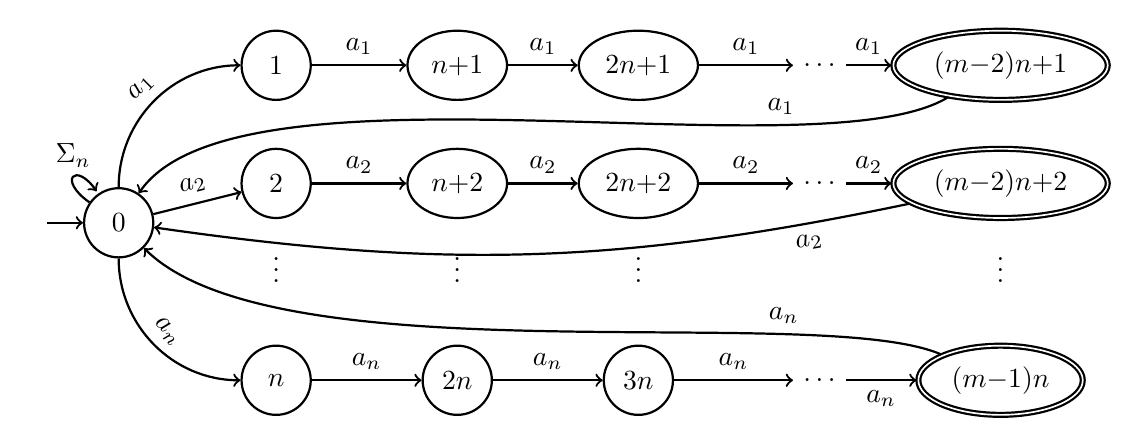
\begin{tikzpicture}[thick,->,initial text={},every state/.style={shape=ellipse}, node distance=2.3cm]
  \node[state,initial]   (0)                    {$0$};
  \node[state]           (1) at ($(0)+(2,2)$)   {$1$};
  \node[state]           (n1) [right of=1]      {$n{+}1$};
  \node[state]           (2n1) [right of=n1]    {$2n{+}1$};
  \node                  (d1) [right of=2n1]    {$\ldots$};
  \node[state,accepting] (m2n1) [right of=d1]   {$(m{-}2)n{+}1$};
  \node[state]           (2) at ($(0)+(2,.5)$) {$2$};
  \node[state]           (n2) [right of=2]      {$n{+}2$};
  \node[state]           (2n2) [right of=n2]    {$2n{+}2$};
  \node                  (d2) [right of=2n2]    {$\ldots$};
  \node[state,accepting] (m2n2) [right of=d2]   {$(m{-}2)n{+}2$};
  \node[state]           (n) at ($(0)+(2,-2)$)  {$n$};
  \node[state]           (2n) [right of=n]      {$2n$};
  \node[state]           (3n) [right of=2n]     {$3n$};
  \node                  (dn) [right of=3n]    {$\ldots$};
  \node[state,accepting] (m1n) [right of=dn]   {$(m{-}1)n$};

  \node (ds1) at ($(0)+(2,-.5)$) {$\vdots$};
  \node (ds2) [right of=ds1] {$\vdots$};
  \node (ds3) [right of=ds2] {$\vdots$};
  \node (ds4) [right of=ds3] {};
  \node ()    [right of=ds4] {$\vdots$};

  \path (0)    edge [out=145,in=125,loop] node [above]                   {$\Sigma_n$} ()
               edge [out=90,in=180]     node [above,sloped]            {$a_1$}      (1)
               edge              node [above,sloped]            {$a_2$}      (2)
               edge [out=270,in=180]             node [above,sloped]            {$a_n$}      (n)
        (1)    edge              node [above]                   {$a_1$}      (n1)
        (n1)   edge              node [above]                   {$a_1$}      (2n1)
        (2n1)  edge              node [above]                   {$a_1$}      (d1)
        (d1)   edge              node [above]                   {$a_1$}      (m2n1)
        (2)    edge              node [above]                   {$a_2$}      (n2)
        (n2)   edge              node [above]                   {$a_2$}      (2n2)
        (2n2)  edge              node [above]                   {$a_2$}      (d2)
        (d2)   edge              node [above]                   {$a_2$}      (m2n2)
        (m2n2) edge [bend left=10]  node [very near start,sloped,below] {$a_2$}      (0)
        (n)    edge              node [above]                   {$a_n$}      (2n)
        (2n)   edge              node [above]                   {$a_n$}      (3n)
        (3n)   edge              node [above]                   {$a_n$}      (dn)
        (dn)   edge              node [below]                   {$a_n$}      (m1n);
%        (m1n)  edge              node [near start,sloped,above] {$a_n$}      (0);

  \draw[->] (m2n1) .. controls ($(m2n1)+(-2.3,-1.4)$) and ($(0)+(1.5,2.2)$) .. (0) node [near start,above] {$a_1$};
  \draw[->] (m1n) .. controls ($(m1n)+(-2.3,1)$) and ($(0)+(2,-2)$) .. (0) node [near start,above] {$a_n$};
\end{tikzpicture}
\end{center}
It is also accepted by the following deterministic B\"uchi automata $\mathcal{B}_{n,m}$.
\begin{center}
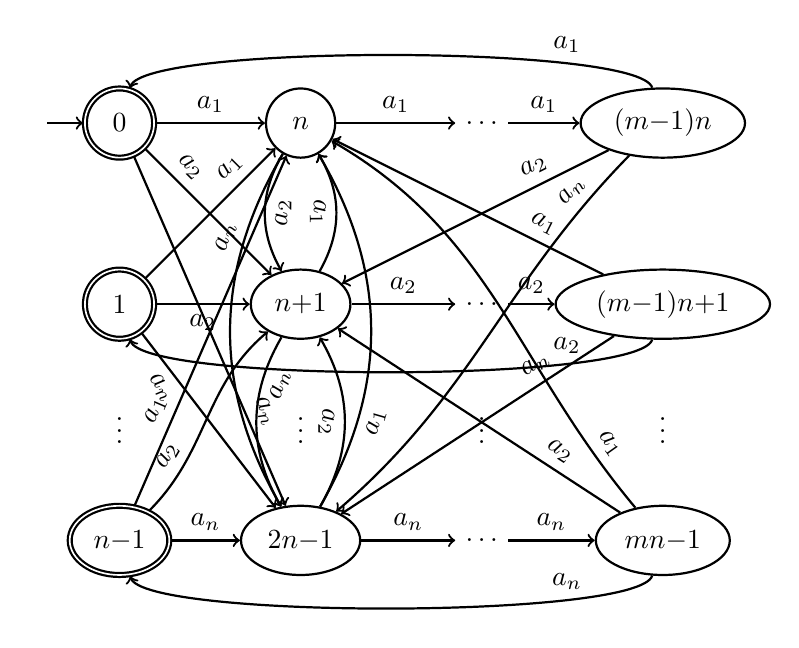
\begin{tikzpicture}[thick,->,node distance=2.3cm,initial text={},every state/.style={shape=ellipse}]
  \node[state,initial,accepting] (0)                        {$0$};
  \node[state,accepting]         (1)      [below of=0]      {$1$};
  \node                          (d1)     [below of=1,node distance=1.5cm]      {$\vdots$}; 
  \node[state,accepting]         (nm1)    [below of=d1,node distance=1.5cm]     {$n{-}1$};
  \node[state]                   (n)      [right of=0]      {$n$};
  \node[state]                   (np1)    [below of=n]      {$n{+}1$};
  \node                          (d2)     [below of=np1,node distance=1.5cm]    {$\vdots$}; 
  \node[state]                   (2nm1)   [below of=d2,node distance=1.5cm]     {$2n{-}1$};
  \node                          (d3)     [right of=n]      {$\ldots$};
  \node                          (d4)     [right of=np1]    {$\ldots$};
  \node                          (d5)     [right of=d2]     {$\vdots$};
  \node                          (d6)     [right of=2nm1]   {$\ldots$};
  \node[state]                   (mm1n)   [right of=d3]     {$(m{-}1)n$};
  \node[state]                   (mm1np1) [below of=mm1n]   {$(m{-}1)n{+}1$};
  \node                          (d7)     [below of=mm1np1,node distance=1.5cm] {$\vdots$}; 
  \node[state]                   (mnm1)   [below of=d7,node distance=1.5cm]     {$mn{-}1$};

  \path[->] (0)    edge node [above] {$a_1$} (n)
            (n)    edge node [above] {$a_1$} (d3)
            (d3)   edge node [above] {$a_1$} (mm1n)
            (1)    edge node [below] {$a_2$} (np1)
            (np1)  edge node [above] {$a_2$} (d4)
            (d4)   edge node [above] {$a_2$} (mm1np1)
            (nm1)  edge node [above] {$a_n$} (2nm1)
            (2nm1) edge node [above] {$a_n$} (d6)
            (d6)   edge node [above] {$a_n$} (mnm1);

  \path[->] (0)      edge                       node [sloped,above,near start]      {$a_2$} (np1)
            (n)      edge [bend right]          node [sloped,below]                 {$a_2$} (np1)
            (mm1n)   edge                       node [sloped,above,near start]      {$a_2$} (np1)
            (1)      edge                       node [sloped,above,near end]        {$a_1$} (n)
            (np1)    edge [bend right]          node [sloped,below]                 {$a_1$} (n)
            (mm1np1) edge                       node [sloped,above,near start]      {$a_1$} (n)
            (0)      edge                       node [sloped,above,near end]        {$a_n$} (2nm1)
            (n)      edge [bend right]          node [sloped,above,near start]        {$a_n$} (2nm1)
            (mm1n)   edge [bend right=5,in=170] node [sloped,above,very near start] {$a_n$} (2nm1)
            (nm1)    edge                       node [sloped,above,near start]      {$a_1$} (n)
            (2nm1)   edge [bend right]          node [sloped,below,near start]      {$a_1$} (n)
            (mnm1)   edge [in=-30,out=130]      node [sloped,above,very near start] {$a_1$} (n)
            (1)      edge                       node [sloped,below,near start]      {$a_n$} (2nm1)
            (np1)    edge [bend right]          node [sloped,below,near start]        {$a_n$} (2nm1)
            (mm1np1) edge                       node [sloped,above,near start]      {$a_n$} (2nm1)
            (nm1)    edge [in=220]              node [sloped,above,near start]      {$a_2$} (np1)
            (2nm1)   edge [bend right]          node [sloped,below]                 {$a_2$} (np1)
            (mnm1)   edge                       node [sloped,above,near start]      {$a_2$} (np1);
            
  \draw[->] (mm1n) .. controls ($(mm1n)+(-.3,1)$) and ($(0)+(.3,1)$) .. (0) node [near start,above] {$a_1$};
  \draw[->] (mm1np1) .. controls ($(mm1np1)+(-.3,-1)$) and ($(1)+(.3,-1)$) .. (1) node [near start,above] {$a_2$};
  \draw[->] (mnm1) .. controls ($(mnm1)+(-.3,-1)$) and ($(nm1)+(.3,-1)$) .. (nm1) node [near start,above] {$a_n$};
\end{tikzpicture}
\end{center}
The synchronous product of $\mathcal{A}_{n,m}$ and $\mathcal{B}_{n,m}$ is a parity game $\mathcal{G}_{n,m}$ in which
every node is owned by player $1$, and the priority of a node $(q,p)$ is given as
\begin{displaymath}
\Omega(q,p) \enspace = \enspace \begin{cases}
2 &,\text{if } p \text{ is accepting,} \\
1 &,\text{if } p \text{ is not accepting and } q \text{ is accepting,} \\
0 &,\text{otherwise.}
\end{cases}
\end{displaymath}
This is the standard encoding of fair simulation as a parity condition \cite{HenzingerKR02,HutagalungLL:LATA13}. This game
encodes the language inclusion problem between an NBA and a DBA. In this case, the game is entirely won by player $0$.

The game $\mathcal{G}_{6,9}$ is generated by
\begin{verbatim}
    ~/pgsolver> bin/langincl 6 9
\end{verbatim}
The second parameter is optional. If it is not given then $m=2$ is chosen by default.


 
%%% Local Variables:
%%% mode: latex
%%% TeX-master: "main"
%%% End:

%\input{./results}

\chapter{Developer's Guide}
\label{chp:dguide}

\input{./develop}

%\appendix

%\chapter{New Algorithms}
%\label{app:newalg}



\cleardoublepage
\pdfbookmark{Bibliography}{bibliography}
\bibliographystyle{alpha}
\bibliography{./literature}

\end{document}



%%% Local Variables:
%%% mode: latex
%%% TeX-master: t
%%% End:
